\documentclass[11pt]{article}
\usepackage[margin=1in]{geometry}
\usepackage{mathpazo}
\usepackage{amsmath,amssymb}
\usepackage{microtype}
\usepackage{booktabs}
\usepackage{graphicx}
\usepackage[dvipsnames]{xcolor}
\usepackage{tikz}
\usetikzlibrary{positioning,arrows.meta,calc,fit,backgrounds}
\usepackage[most]{tcolorbox}
\usepackage{enumitem}
\usepackage{listings}
\usepackage[font=small,labelfont=bf]{caption}
\usepackage{hyperref}
\hypersetup{colorlinks=true,linkcolor=MidnightBlue,citecolor=MidnightBlue,urlcolor=MidnightBlue}
\usepackage{cleveref}
\urlstyle{tt}
\def\UrlBreaks{\do\_\do/\do.}
\newcommand{\file}[1]{\nolinkurl{#1}}
\newcommand{\code}[1]{\texttt{#1}}
\newcommand{\mhh}{m_{hh}}
\newcommand{\bw}{\boldsymbol{\omega}}
\newcommand{\bp}{\boldsymbol{p}}
\newcommand{\bx}{\boldsymbol{x}}
\newcommand{\data}{\mathcal{D}}

\definecolor{trainable}{HTML}{1B6CA8}
\definecolor{physics}{HTML}{2E933C}
\definecolor{datac}{HTML}{7B4EA3}
\definecolor{warn}{HTML}{C0392B}

\newtcolorbox{keyidea}[1][]{enhanced,breakable,colback=physics!6,colframe=physics!70!black,
  fonttitle=\bfseries,title={#1},boxrule=0.6pt,arc=2pt,left=6pt,right=6pt}
\newtcolorbox{aside}[1][]{enhanced,breakable,colback=trainable!5,colframe=trainable!70!black,
  fonttitle=\bfseries,title={#1},boxrule=0.6pt,arc=2pt,left=6pt,right=6pt}
\newtcolorbox{assume}[1][]{enhanced,breakable,colback=datac!5,colframe=datac!70!black,
  fonttitle=\bfseries,title={#1},boxrule=0.6pt,arc=2pt,left=6pt,right=6pt}
\newtcolorbox{watch}[1][]{enhanced,breakable,colback=warn!5,colframe=warn!70!black,
  fonttitle=\bfseries,title={#1},boxrule=0.6pt,arc=2pt,left=6pt,right=6pt}
\setlist{itemsep=2pt,topsep=3pt}
\setlength{\emergencystretch}{3em}

\lstset{language=Python, basicstyle=\ttfamily\small, columns=fullflexible,
  keepspaces=true, commentstyle=\color{physics!70!black}\itshape,
  keywordstyle=\color{trainable!90!black}\bfseries, stringstyle=\color{datac},
  showstringspaces=false, frame=single, rulecolor=\color{gray!40},
  backgroundcolor=\color{gray!3}, xleftmargin=4pt, xrightmargin=4pt,
  aboveskip=6pt, belowskip=6pt}

\title{\textbf{The Bayesian neural network with the Poisson likelihood}\\[4pt]
\large Results of the run \texttt{runs/BNN\_poisson} (10\% of the training spectra)}
\date{October 30, 2026}

\begin{document}
\maketitle

\begin{abstract}
\noindent
The second BNN run used the experimental \code{'poisson'} likelihood, a Gaussian with
the known POWHEG noise of each bin (the counterpart of the CHI2 loss), on 10\% of the
training spectra, with a long warm-up (1,500 iterations) and long trajectories (500
leapfrog steps), started from \file{runs/L1Loss}. On the 1,000 holdout spectra it is the
most accurate model so far: the mean $\chi^2$ per bin between 255 and 555~GeV, the region
that has been the model's weakness since October 26, falls from 8.4 (the L1 model) and 3.6
(the Laplace BNN) to 1.7, and spectra with $\chi^2/N > 5$ fall from 4.9\% to 1.0\%. Its
bands are close to calibrated: the pull of POWHEG against the BNN has a standard
deviation of 1.04 above 555~GeV and 1.19 below. Most of this comes from a more accurate
mean rather than from the band. The chain is not yet fully settled, and the warm-up spent
85\% of its iterations with a tiny step size because the mass matrix was set only once;
\file{hmc.py} is being changed to fix that (\cref{sec:next}). The three models disagree
by a factor of two on the Standard Model prediction just above threshold, far beyond any
one chain's band.
\end{abstract}

\begin{keyidea}[The main findings]
\begin{enumerate}
  \item \textbf{Much better near threshold.} Mean $\chi^2$ per bin at 255--555 GeV:
    8.4 (L1) $\to$ 3.6 (Laplace BNN) $\to$ \textbf{1.7} (Poisson BNN), with only a tenth of
    the training spectra. Median $\chi^2/N$ 1.09; negative predictions 0.006\%.
  \item \textbf{An optimisation effect again.} The first sample is as good as the mean:
    the warm-up acted as a full-batch optimiser of $\chi^2$, starting from the L1 solution.
    This is where the CHI2 loss, trained from scratch with mini-batches, failed. A
    two-stage training (L1, then full-batch $\chi^2$) may give the same result without HMC.
  \item \textbf{Nearly calibrated.} Standard deviation of the pull 1.08 overall (ideal 1),
    93.8\% of bins with $|z| < 2$ (ideal 95\%). The band is 5.6\% of the POWHEG noise
    (median), about $\sqrt{10}$ times wider than in run 1, as expected for a tenth of the
    data.
  \item \textbf{The sampler: better mixing, but a wasteful warm-up and some drift.} ESS of
    the monitored predictions 137 and 61 (run 1: 123 and 5). But $U$ and the prior
    precisions of the large hidden-weight groups were still drifting during sampling.
  \item \textbf{A warning.} At the SM point and 262.5~GeV the three models give
    $3.1$, $4.3$ and $6.1 \times 10^{-5}$~pb; each chain's own band is $\pm 2$--$3\%$.
\end{enumerate}
\end{keyidea}

\tableofcontents

% ===========================================================================
\section{The run}

\begin{center}
\small
\begin{tabular}{ll}
\toprule
setting & value\\
\midrule
likelihood & \code{'poisson'}: Gaussian, known variance $\sigma_k^2 = (f_k + \sigma_\text{tot}/N_\text{eff})\,\sigma_\text{tot}/N_\text{eff}$, $N_\text{eff} = 38{,}024$\\
prior & Neal's hierarchical prior, 16 groups, $\tau_g$ Gibbs-sampled\\
warm start & \file{runs/L1Loss/dihiggs_params.pth}\\
training rows & 27,183: 10\% of the training spectra (about 340), all their bins\\
iterations & 1,500 warm-up + 500 saved\\
leapfrog steps & $L = 500$ (jittered by $\pm 10\%$)\\
chains & 1, seed 42\\
\bottomrule
\end{tabular}
\end{center}

\noindent The folder \file{runs/BNN_poisson/chain_1/} is left over from an earlier,
aborted attempt and holds no samples; it is harmless (\code{hmc.BNN} reads only sample
files) but can be deleted. The 500 samples were evaluated with \code{hmc.BNN} on all
1,000 holdout spectra, as in \file{bnn_run1.pdf}.

% ===========================================================================
\section{The sampler}
\label{sec:sampler}

\begin{figure}[h]
\centering
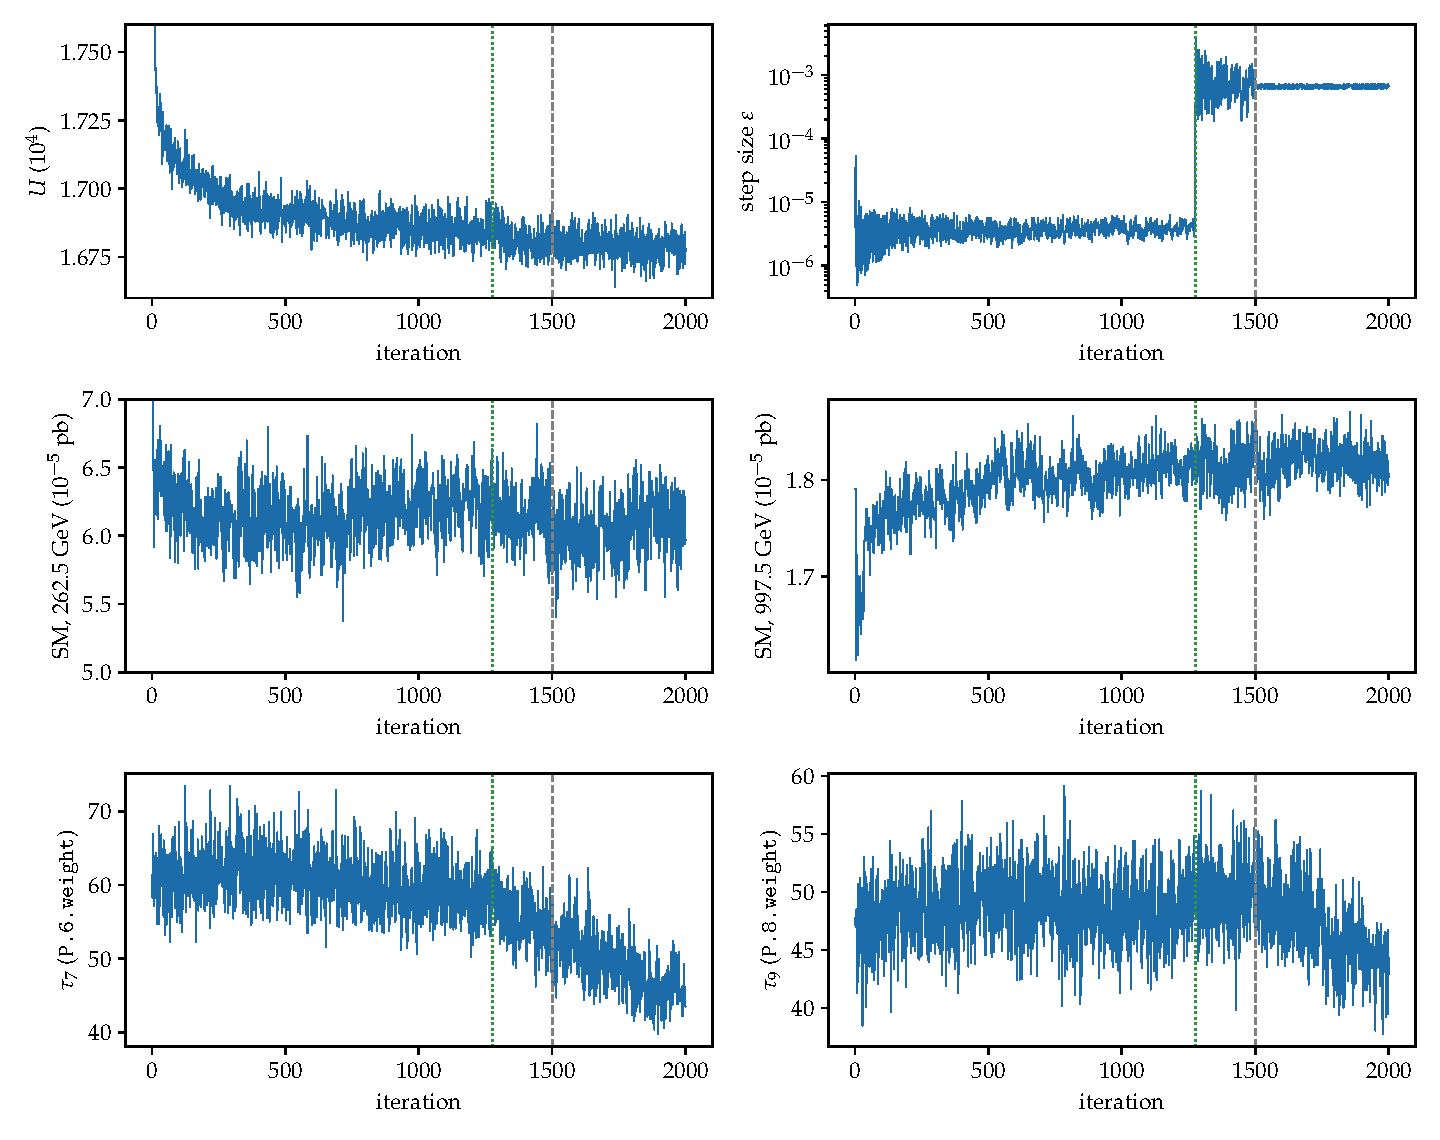
\includegraphics[width=\textwidth]{fig2_traces.pdf}
\caption{Traces of $U$, the step size, the two monitored predictions (the SM point at 262.5
and 997.5 GeV), and the prior precisions of the weights of the fourth and fifth hidden
layers. Green dotted line: the mass matrix is set (iteration 1,275); grey dashed line: end
of the warm-up.}
\label{fig:traces}
\end{figure}

\begin{center}
\small
\begin{tabular}{lrrl}
\toprule
quantity & ESS (of 500) & split-$\hat R$ & verdict\\
\midrule
$U$ & 181 & 1.02 & still drifting down slowly\\
SM prediction, 262.5 GeV & 137 & 1.04 & acceptable\\
SM prediction, 997.5 GeV & 61 & 1.00 & acceptable (run 1: 5)\\
$\tau_g$, biases and first/last layers & 340--520 & 1.00--1.02 & mix well\\
$\tau_3, \tau_5, \tau_7, \tau_9, \tau_{13}$ (large weight matrices) & 7--23 & 1.10--1.44 & \textbf{drifting}\\
\bottomrule
\end{tabular}
\end{center}

\paragraph{The descent.} $U$ starts at 27,700 and falls to 17,700 within ten iterations
(the first accepted trajectory has $\Delta H = -1{,}130$), then keeps falling slowly: to
17,050 by iteration 100 and to about 16,780 at the end. During sampling it still falls by
about 5 per 100 iterations, against an iteration-to-iteration fluctuation of 47, which is
what $d = 3{,}944$ parameters give ($\sqrt{d/2} \approx 44$). The chain is close to
equilibrium, but not there.

\paragraph{The wasted warm-up.} \Cref{fig:traces} shows the cause. \file{hmc.py} sets the
mass matrix once, at 85\% of the warm-up. Until then every parameter has unit mass, and the
step size must suit the most tightly constrained direction: it was about
$3 \times 10^{-6}$ for 1,275 iterations. At iteration 1,275 the mass matrix was set from
the variance of the parameters over iterations 225--1,275, and the step size jumped about
200-fold, to $6.6 \times 10^{-4}$. Even then a trajectory lasts only
$\varepsilon L \approx 0.33$ posterior standard deviations, and the acceptance rate during
sampling, 0.94, is well above the target of 0.8: the step size could have been larger,
but the step-size tuning had only 225 iterations after the mass matrix changed.

\paragraph{The drift of the hidden-layer precisions.} Once the chain could move
(after iteration 1,275), the precisions of the large weight matrices began to drift:
$\tau_7$ falls from about 60 to 45, $\tau_9$ from about 50 to 43, i.e.\ the weights of
those layers grow. Their ESS of 7--23 reflects that drift, not slow mixing about a fixed
level. The chain is still relaxing in the directions that the first 1,275 iterations
could not explore.

% ===========================================================================
\section{Accuracy on the holdout spectra}
\label{sec:accuracy}

\begin{center}
\small
\begin{tabular}{lccc}
\toprule
& L1Loss (start) & BNN, Laplace (run 1) & BNN, Poisson (run 2)\\
\midrule
median $\chi^2/N$ & 1.171 & 1.127 & \textbf{1.092}\\
spectra with $\chi^2/N > 2$ & 13.6\% & 9.2\% & \textbf{4.5\%}\\
spectra with $\chi^2/N > 5$ & 4.9\% & 2.5\% & \textbf{1.0\%}\\
mean $\chi^2$ per bin, 255--555 GeV & 8.4 & 3.6 & \textbf{1.7}\\
mean $\chi^2$ per bin, above 555 GeV & 1.20 & 1.16 & \textbf{1.11}\\
mean $|$residual$|$ ($10^{-3}$ pb) & 2.98 & \textbf{2.92} & 3.04\\
negative predictions & 0.18\% & 0.07\% & \textbf{0.006\%}\\
\bottomrule
\end{tabular}
\end{center}

\begin{figure}[h]
\centering
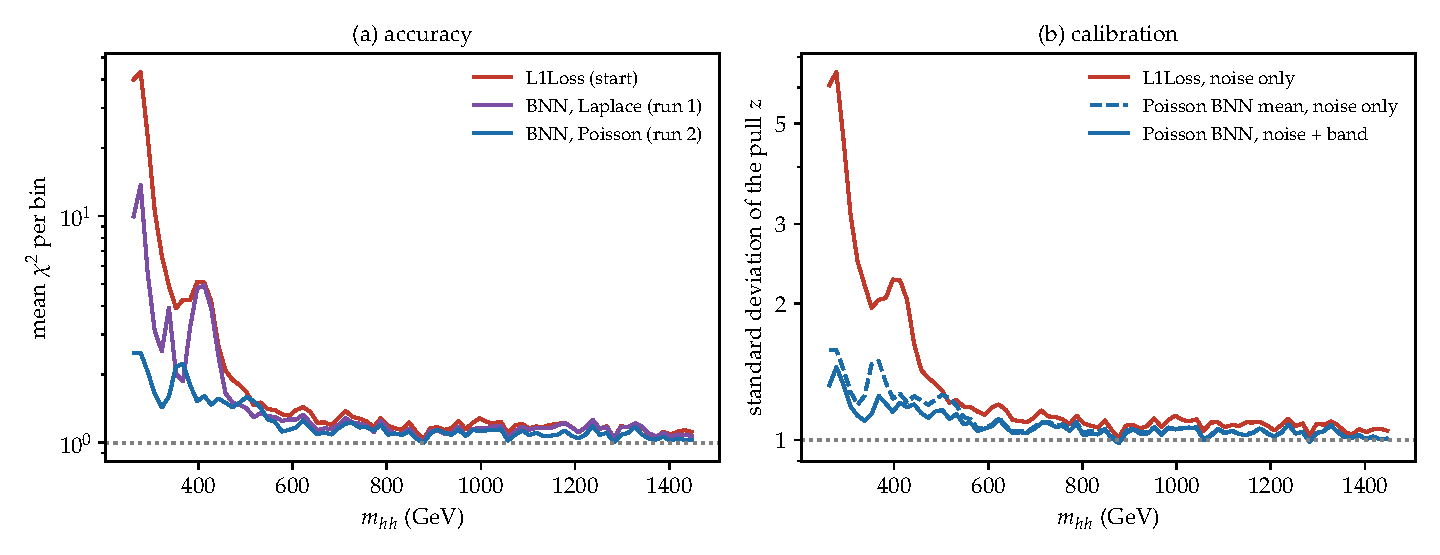
\includegraphics[width=\textwidth]{fig2_holdout.pdf}
\caption{(a) Mean $\chi^2$ per bin over the 1,000 holdout spectra against $\mhh$. (b)
Standard deviation of the pull $z$ against $\mhh$: the L1 model and the Poisson BNN mean
with the POWHEG noise alone in the denominator, and the Poisson BNN with noise and band.}
\label{fig:holdout}
\end{figure}

\noindent The improvement is concentrated near threshold (\cref{fig:holdout}a), where
the Poisson BNN is within a factor of two of the noise everywhere. The one measure on
which it is worse, the mean absolute residual, is the one the L1 loss optimises: $\chi^2$
measures each error in units of that bin's noise and so gives up a little in the large
bins, where the absolute errors are largest.

\begin{keyidea}[Optimisation, not averaging; and a cheap test]
The first sample (median $\chi^2/N$ 1.099) is as good as the mean (1.092). As in run 1, the
gain comes from the warm-up, which here acted as a full-batch optimiser of $\chi^2$
starting from the L1 solution. The CHI2 loss failed when trained from scratch with
mini-batches (\file{dihiggs_report.pdf}); started from the L1 solution, with full-data
gradients, it works, and on a tenth of the data. A two-stage training in
\file{heft_train.ipynb}, L1 followed by a full-batch $\chi^2$ fine-tune, may give the same
accuracy without HMC. It is the cheapest candidate for a production fix of the threshold
region.
\end{keyidea}

% ===========================================================================
\section{Calibration}
\label{sec:calibration}

As in the ensemble plan, form at every holdout bin the pull
$z = (t - \bar f)/\sqrt{\sigma_k^2 + s^2}$, where $t$ is POWHEG, $\bar f$ the BNN mean,
$\sigma_k$ the POWHEG noise and $s$ the posterior standard deviation. If the band accounts
for the model's error, $z$ has standard deviation 1.

\begin{center}
\small
\begin{tabular}{lccc}
\toprule
& s.d.\ of $z$, all & s.d.\ of $z$, 255--555 GeV & $|z| < 2$\\
\midrule
L1Loss, noise only & 1.74 & 2.88 & \\
Poisson BNN mean, noise only & 1.12 & 1.31 & \\
Poisson BNN, noise and band & \textbf{1.08} & \textbf{1.19} & \textbf{93.8\%} (ideal 95\%)\\
\bottomrule
\end{tabular}
\end{center}

\noindent Above 555~GeV the standard deviation of $z$ is 1.04. The band's median width is
5.6\% of the POWHEG noise (9.2\% near threshold, 4.7\% above); 10\% of POWHEG values lie
inside the 95\% credible band (run 1: 4.2\%). The comparison of the last two rows shows
that most of the improvement in calibration comes from the more accurate mean; the band
accounts for about a third of the remaining excess near threshold. With all the data, the
band will narrow by about $\sqrt{10}$, so the calibration of the full-data run cannot be
assumed from this one.

% ===========================================================================
\section{A warning about the threshold}
\label{sec:threshold}

\begin{figure}[h]
\centering
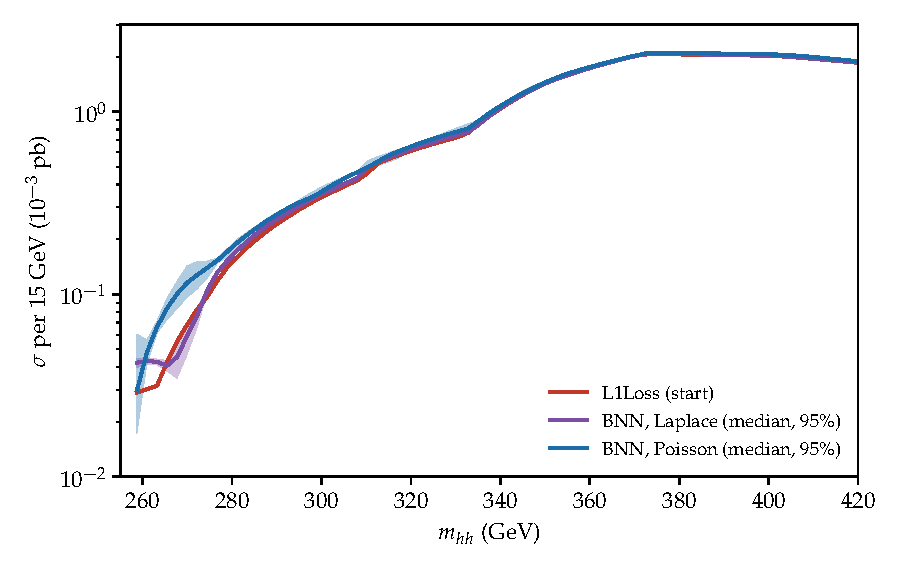
\includegraphics[width=0.65\textwidth]{fig2_sm.pdf}
\caption{The Standard Model spectrum,
$(\kappa_\lambda, c_t, c_{tt}, c_{ggh}, c_{gghh}) = (1, 1, 0, 0, 0)$, near threshold:
the L1 model, and the median and 95\% band of the two BNNs.}
\label{fig:sm}
\end{figure}

At the SM point in the first bin above threshold (262.5 GeV) the three models give
$3.1$, $4.3$ and $6.1 \times 10^{-5}$~pb (L1, Laplace BNN, Poisson BNN), a factor of two,
while each BNN's own 95\% band is a few per cent wide (\cref{fig:sm}). The cross section
there is about $10^{-2}$ of its peak, and with the L1 and Laplace likelihoods it carries
almost no weight in the fit. The Poisson likelihood weights it by its precision, which is
why it moves most. Within each run the band is narrow; across runs the answer depends on
the likelihood. No single chain's band reflects this kind of uncertainty, and any use of the
model at threshold should keep it in mind. (Whether the SM point is well inside the region
covered by the training points is worth checking.)

% ===========================================================================
\section{Next steps}
\label{sec:next}

\begin{enumerate}
  \item \textbf{A better warm-up in \file{hmc.py}} (being implemented): update the mass
    matrix several times during the warm-up, in windows of growing length, restarting the
    step-size tuning after each update and continuing it until the end of the warm-up, as
    Stan does. The first update then comes after about a quarter of the warm-up rather than
    at 85\%.
  \item \textbf{Thinning for users} (being implemented): select every $K$-th saved sample,
    with $K$ suggested from the autocorrelation times of the trace, and write the selection
    as a small, self-contained ensemble of nearly independent draws.
  \item \textbf{Repeat this run} with the improved \file{hmc.py}, changing only
    \code{N\_LEAPFROG} (your plan), then examine it, then a run on all the data.
  \item \textbf{Test the two-stage training} (L1, then full-batch $\chi^2$) in
    \file{heft_train.ipynb}.
  \item \textbf{For the bootstrap ensemble:} if two-stage training works, train the
    members that way, or the threshold bias will dominate the comparison.
  \item \textbf{Small notebook fixes} (being made): skip the noise-scale panel of the trace
    figure for the Poisson likelihood, where there is no noise scale, and show the step
    size instead; limit the y-range of the relative-band panels.
\end{enumerate}

\end{document}
